%
% schuhbaendel.tex
%
% (c) 2018 Prof Dr Andreas Müller, Hochschule Rapperswil
%
\documentclass[tikz]{standalone}
\usepackage{times}
\usepackage{amsmath}
\usepackage{txfonts}
\usepackage[utf8]{inputenc}
\usepackage{graphics}
\usepackage{color}
\usepackage{pifont}
\usetikzlibrary{arrows,intersections,math,calc}
\begin{document}

\def\punkt#1{
        \fill[color=white] #1 circle[radius=0.08];
        \draw #1 circle[radius=0.08];
}

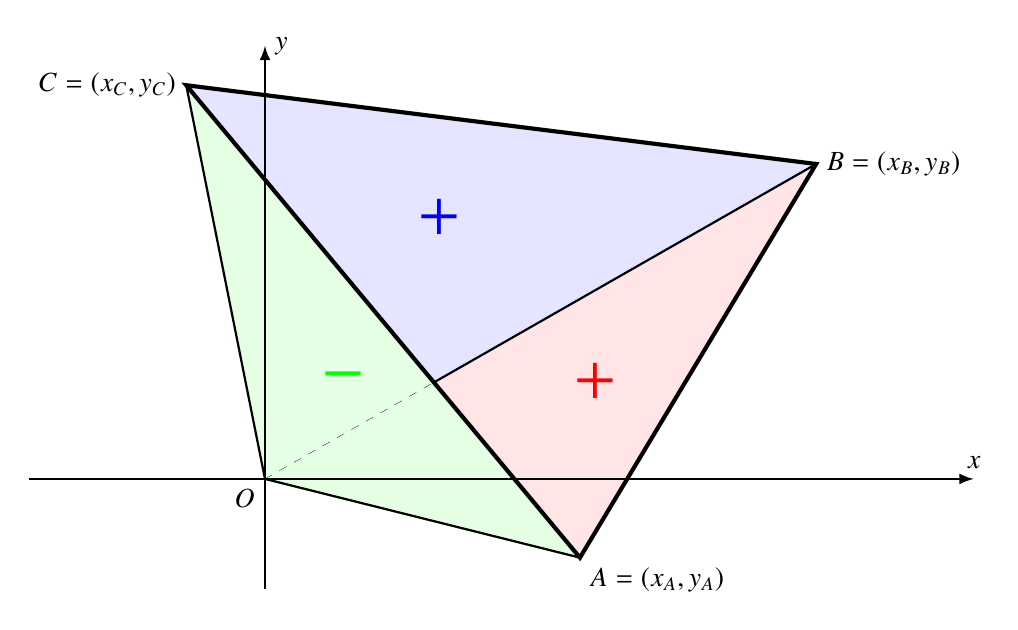
\begin{tikzpicture}[>=latex,thick]

\coordinate (O) at (0,0);
\coordinate (A) at (4,-1);
\coordinate (B) at (7,4);
\coordinate (C) at (-1,5);

\fill[color=red!10] (O)--(A)--(B)--cycle;
\fill[color=blue!10] (O)--(B)--(C)--cycle;
\draw (O)--(B);
\fill[color=green!10] (O)--(C)--(A)--cycle;
\draw (O)--(A);
\draw (O)--(C);
\draw[line width=0.1pt,dashed] (O)--(B);

\draw[line width=1.5pt] (A)--(B)--(C)--cycle;

\draw[->] (-3.0,0)--(9.0,0) coordinate[label=$x$];
\draw[->] (0,-1.4)--(0,5.5) coordinate[label={right:$y$}];

\node[color=red] at ($(O)+0.35*(A)+0.4*(B)$) {\Huge$+$};
\node[color=blue] at ($(O)+0.37*(B)+0.37*(C)$) {\Huge $+$};
\node[color=green] at ($(O)+0.333*(A)+0.333*(C)$) {\Huge$-$};

\punkt{(A)} \node at (A) [below right] {$A=(x_A,y_A)$};
\punkt{(B)} \node at (B) [right] {$B=(x_B,y_B)$};
\punkt{(C)} \node at (C) [left] {$C=(x_C,y_C)$};
\punkt{(O)} \node at (O) [below left] {$O$};

\end{tikzpicture}

\end{document}

